\documentclass{article}
\usepackage[utf8]{inputenc}
\usepackage[margin=0.6in, a4paper]{geometry} 
\usepackage{xcolor}
\usepackage{hyperref}
\usepackage{qrcode}
\usepackage{graphicx}

% --- ตั้งค่าสีสำหรับธีม CMD และ IDE ---
\definecolor{CMD_Black}{HTML}{0C0C0C} 
\definecolor{CMD_Gray}{HTML}{CCCCCC}  
\definecolor{VSCodeBG}{HTML}{1E1E1E}  
\definecolor{CommentGreen}{HTML}{6A9955}
\definecolor{KeywordBlue}{HTML}{569CD6}
\definecolor{StringOrange}{HTML}{CE9178}

% บังคับให้เป็น Font Monospace (ฟอนต์โค้ด) ทั้งเอกสาร
\renewcommand{\familydefault}{\ttdefault}
\hypersetup{colorlinks=true, linkcolor=KeywordBlue, urlcolor=KeywordBlue}

\begin{document}

% ==========================================
% [ANIMATION FRAME 1] : หน้าจอว่างๆ มีเคอร์เซอร์กะพริบ
% ==========================================
\pagecolor{CMD_Black}
\color{CMD_Gray}

\noindent Microsoft Windows [Version 10.0.19045.4291]\\
(c) Microsoft Corporation. All rights reserved.\\
\\
C:\textbackslash Users\textbackslash ComEn\_Student> \_ % เคอร์เซอร์กะพริบตอนแรก

% ==========================================
% [ANIMATION FRAME 2] : พิมพ์คำสั่ง /info สำเร็จ
% ==========================================
\newpage
\noindent Microsoft Windows [Version 10.0.19045.4291]\\
(c) Microsoft Corporation. All rights reserved.\\
\\
C:\textbackslash Users\textbackslash ComEn\_Student> \textbf{/info} \\

% ==========================================
% [ANIMATION FRAME 3] : ระบบขึ้นว่ากำลัง Loading...
% ==========================================
\newpage
\noindent Microsoft Windows [Version 10.0.19045.4291]\\
(c) Microsoft Corporation. All rights reserved.\\
\\
C:\textbackslash Users\textbackslash ComEn\_Student> \textbf{/info} \\
\\
\textcolor{white}{[SYSTEM] Accessing personal\_data.db...}\\
\textcolor{white}{[SYSTEM] Decrypting student\_profile...}\\
\textcolor{white}{[SYSTEM] Loading resources... [||||||||||||||||||] 100\%}\\
\textcolor{white}{[SYSTEM] Redirecting to terminal\_interface.exe...}

% ==========================================
% [FINAL PAGE] : หน้าข้อมูลหลัก (ธีม VS Code)
% ==========================================
\newpage
\pagecolor{VSCodeBG}
\color{white}

\noindent
\textcolor{CommentGreen}{// Profile initialization... Complete} \\
\textcolor{CommentGreen}{// Assets loaded: Me.jpg, Idol.jpg} \\

% โซนแสดงรูปคู่ (วางคู่กันซ้าย-ขวา แบบเนี๊ยบๆ)
\begin{center}
    \begin{minipage}{0.35\textwidth}
        \centering
        \framebox{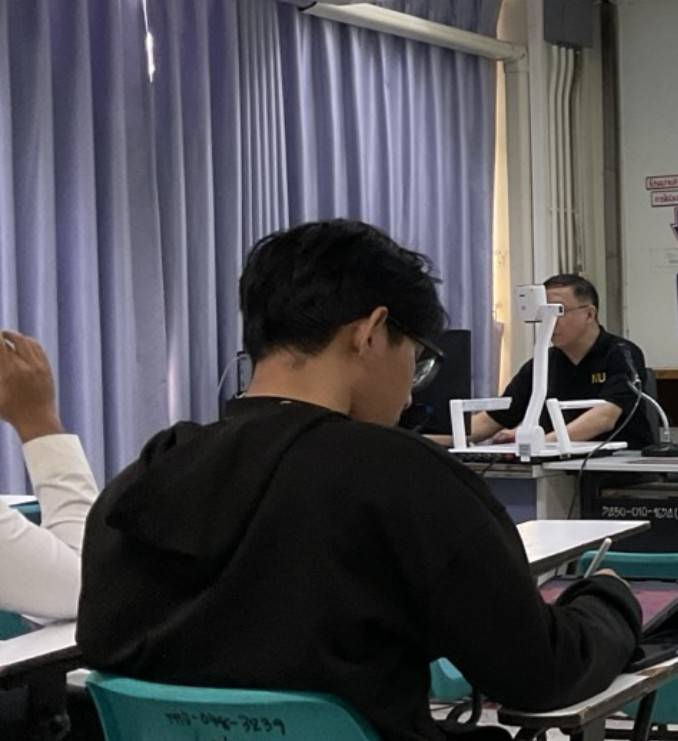
\includegraphics[width=0.9\textwidth]{Me.jpg}} \\
        \footnotesize \textcolor{CommentGreen}{// [FILE]: Me.jpg}
    \end{minipage}
    \begin{minipage}{0.35\textwidth}
        \centering
        \framebox{
\includegraphics[width=0.9\textwidth]{Idol.jpg}} \\
        \footnotesize \textcolor{CommentGreen}{// [FILE]: Idol.jpg}
    \end{minipage}
\end{center}

\vspace{0.1in}
\begin{center}
    \Huge \textbf{\textcolor{KeywordBlue}{class}} \textcolor{StringOrange}{ComEn\_Student} \{
\end{center}

\normalsize
\vspace{0.15in}

% =========================================================
% >>>  [โซนเติมข้อมูลของคุณ] เติมในเครื่องหมายคำพูด "..." ได้เลยครับ <<<
% =========================================================
\noindent
\hspace{20pt} \textbf{name:} \textcolor{StringOrange}{"Wongsarthon seabuangam "}, \\
\hspace{20pt} \textbf{Id:} \textcolor{StringOrange}{"68364678"}, \\
\hspace{20pt} \textbf{Gender:} \textcolor{StringOrange}{"Male 19yo"}, \\
\hspace{20pt} \textbf{major:} \textcolor{StringOrange}{"Computer Engineering Year 2"}, \\
\hspace{20pt} \textbf{Occupation:} \textcolor{StringOrange}{"College student"}, \\
\hspace{20pt} \textbf{Address:} \textcolor{StringOrange}{"Lat,15.81268300494503, Lng,100.54093200848286"} \\
\hspace{20pt} \textbf{For My lecturer:} \textcolor{StringOrange}{"Life Skill Sec 3"}, \\
\noindent \textbf{\}}

\vspace{0.2in}

\noindent
\textcolor{CommentGreen}{// Running extension: ./load\_extra\_details.sh} \\
\textcolor{KeywordBlue}{student@ComEn} \textcolor{CMD_Gray}{\$ cat more\_info.json} \\

\vspace{0.1in}
\noindent \{ \\
\hspace{20pt} \textbf{learning\_inspiration:} \textcolor{StringOrange}{"Passion from motivation and discipline right? I just search showcases on Google like TailwindCSS showcase."}, \\
\hspace{20pt} \textbf{goals:} \textcolor{StringOrange}{"Be better than yesterday, Bro."}, \\
\hspace{20pt} \textbf{skills:} \textcolor{KeywordBlue}{ClickHere>>>} \href{https://github.com/Neo-woupier}{\textcolor{StringOrange}{Neo-woupier (NruNew)}} \textcolor{KeywordBlue}{<<<<<<ClickHere}, \\
\hspace{20pt} \textbf{personality:} \textcolor{StringOrange}{"Introvert, funny, loves making weird jokes, but work comes first."}, \\
\hspace{20pt} \textbf{technology:} [\textcolor{KeywordBlue}{"Web"}, \textcolor{KeywordBlue}{"Postman"}, \textcolor{KeywordBlue}{"Nmap"}, \textcolor{KeywordBlue}{"Burp Suite"}], \\
\hspace{20pt} \textbf{hobby:} \textcolor{StringOrange}{"Play games (Like a normal person)"} \\
\noindent \} \\

\vspace{0.2in}

% --- ส่วน Life Style ที่ขอแบบเด่นๆ ---
\begin{center}
    \Large \textbf{\textcolor{KeywordBlue}{[LIFE\_STYLE]} ==} \textcolor{StringOrange}{"Just come to find my style (:\_;\}\})"}
\end{center}

\vfill
% ==========================================
% [EXTRA PAGE] : System Logs & True Passion
% ==========================================
\newpage
\pagecolor{CMD_Black}
\color{CMD_Gray}

\noindent
\textcolor{white}{[root@ComEn\_Student]\# dmesg | tail -n 15} \\
\\
\texttt{[    0.000000] Linux version 6.x.x-ComEn (student@build) (gcc version 11.2.0)} \\
\texttt{[    0.045123] Command line: BOOT\_IMAGE=/boot/vmlinuz root=UUID=... ro quiet splash} \\
\texttt{[    0.123456] \textcolor{CommentGreen}{[  OK  ]} Started Hardware Initialization.} \\
\texttt{[    0.456789] \textcolor{CommentGreen}{[  OK  ]} Reached target System Initialization.} \\
\texttt{[    0.890123] Mounting Core Life Modules...} \\
\texttt{[    1.002345] \textcolor{StringOrange}{[ WARN ]} Low balance detected in bank\_account.service.} \\
\texttt{[    1.005678] \textcolor{StringOrange}{[ WARN ]} High pressure detected in family\_expectations.conf.} \\
\texttt{[    1.123456] \textcolor{KeywordBlue}{[ INFO ]} Rerouting power to discipline.service.} \\
\texttt{[    1.500000] \textcolor{CommentGreen}{[  OK  ]} Survival\_Mode.sh executed successfully.} \\
\texttt{[    1.800000] Starting Deep\_Reflection\_Daemon...} \\
\texttt{[    2.000000] Scanning for 'Passion' module... \textcolor{red}{[NOT FOUND]}} \\
\texttt{[    2.100000] Overriding system panic... Compiling alternative drive.} \\

\vspace{0.6in}

% --- The Passion Statement ---
\begin{center}
    \textcolor{KeywordBlue}{================================================================} \\
    \vspace{0.15in}
    \Large \textbf{\textcolor{white}{>> SYSTEM OVERRIDE: DEFINING PASSION <<}} \\
    \vspace{0.2in}
    \normalsize
    \textcolor{StringOrange}{
    "Just a kid trying to level up in life. \\
    When your background, family, and financial constraints \\
    leave absolutely no room for surrender... \\
    Even if you don't have a specific 'passion', \\
    the sheer refusal to give up \textbf{BECOMES} the passion itself."
    } \\
    \vspace{0.2in}
    \textcolor{KeywordBlue}{================================================================}
\end{center}

\vfill
\noindent
\textcolor{CommentGreen}{root@ComEn\_Student:\textasciitilde\#} \_

% ==========================================
% [PAGE 4] : README & PROJECT REQUIREMENTS
% ==========================================
\newpage
\pagecolor{white} % เปลี่ยนเป็นพื้นหลังขาวคลีนแบบสไตล์เอกสารทั่วไป
\color{black}     % ตัวหนังสือสีดำปกติ

\noindent
\Large\textbf{README.md} \\
\normalsize
\textcolor{gray}{Last updated: \today} \\
\rule{\textwidth}{0.4pt} % เส้นคั่นแนวนอนสวยๆ

\vspace{0.2in}

\noindent
\large\textbf{1. Project Description} \\
\normalsize
This resume/portfolio document was crafted entirely using \LaTeX\ source code. It demonstrates typesetting skills, structured layout configuration, and precise package implementation without the use of visual drag-and-drop editors.

\vspace{0.2in}

\noindent
\large\textbf{2. System Requirements \& Dependencies} \\
\normalsize
To compile and render this project successfully, the following \LaTeX\ environment configurations and packages are required:

\begin{itemize}
    \item \textbf{\TeX\ Distribution:} TeX Live (2020 or later), MiKTeX, or Overleaf (pdfLaTeX compiler).
    \item \textbf{Core Packages:}
    \begin{itemize}
        \item \texttt{xcolor} -- For system terminal color themes and styling.
        \item \texttt{hyperref} -- For hyperlinking GitHub profiles and contact links.
        \item \texttt{qrcode} -- For generating scannable portfolio links.
        \item \texttt{graphicx} -- For handling external profile and project assets.
    \end{itemize}
    \item \textbf{Font Configuration:} Standard \LaTeX\ typewriter fonts (\texttt{\textbackslash texttt}) for visual terminal emulation.
\end{itemize}

\vspace{0.2in}

\noindent
\large\textbf{3. Compilation Guide} \\
\normalsize
1. Upload all project assets (\texttt{main.tex}, \texttt{Me.jpg}, \texttt{Idol.jpg}) to the root directory. \\
2. Set the primary compiler engine to \textbf{pdfLaTeX}. \\
3. Click \textbf{Recompile}. The output will be generated as a standardized document.

\vspace{0.4in}
\begin{center}
    \small\textcolor{gray}{--- End of Project Specifications ---}
\end{center}

\vfill
\noindent
\textcolor{CommentGreen}{Process finished with exit code 0}

\end{document}